\chapter{Sistemas de Detecção de Quedas}
\label{cap:sistemasRecomendacao}

Um \ac{FDS}, pode ser descrito com um dispositivo de apoio, cujo principal objetivo é alertar o usuário em um evento de queda \citep{igual2013challenges}. Este tipo de sistema pode ser desenvolvido de diversas formas é pode está tanto embarcado em um dispositivo Wearable como um smartwatch ou se basear em um sistema de monitoramento utilizando câmeras.

Com o uso de sistemas de detecção de quedas é possível que o usuário tenha o seu medo de cair reduzido, e dependendo da solução que foi desenvolvida, possa ser socorrido de maneira muito mais rápida, caso necessário. Um individuo que que já sofreu uma queda, pode desenvolver uma sindrome chamada \ac{FOF}, que pode levar a perda da capacidade de se realizar atividades rotinieiras, como passear em um parque, ou assistir um filme em família \citep{legters2002fear}.

As seções desse capítulo são organizadas da seguinte maneira: A seção \ref{sec:fall_definition} define o conceito de quedas e expõe os diversos estados da mesma; A \ref{sec:fall_system_types} irá demonstrar os 3 diferentes tipos de sistemas de detecção quedas mais populares; A seção \ref{sec:sensors} irá demonstrar os principais sensores utilizados nos sistemas de detecção de quedas; A seção  Por fim, a seção \ref{sec:fds_examples}  irá mostrar exemplos de aplicações que realizam a detecção de quedas. 



\section{Definição de Queda}
\label{sec:fall_definition}
De forma geral, podemos definir uma queda como um evento súbito e involuntário, onde o indivíduo de uma posição em pé ou sentado, passa a ocupar uma posição integral ou parcialmente deitada (Horizontal). Na busca por uma definição mais formal, em 1987, o Kellog International Working Group on the prevention of falls, descreveu uma queda como "Vir ao chão ou algum nível mais baixo, sem a intenção como consequência de um golpe violento, perda de consciência, ou início súbito de paralisia como no caso de um acidente vascular cerebral ou um ataque epiléptico"  \citep{igual2013challenges}. Quando analisamos uma queda através das pesperctiva da aceleração do movimento, ela pode ser dividida em etapas descritas na imagem \ref{fig:fall_states}. Estas 4 etapas são as seguintes:



\begin{figure}[ht]
	\centering
	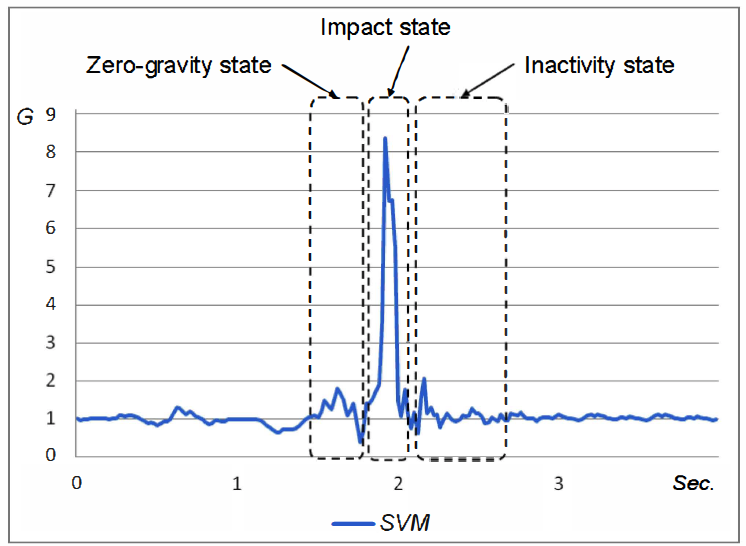
\includegraphics[scale=0.4]{imagens/fall_states.png}
	\caption{Etapas de uma queda \citep{hsieh2014wrist}.}
	\label{fig:fall_states}
\end{figure} 


\begin{itemize}
	\item{\textbf{Período Anterior a Queda (Pre-Fall)}: Durante este período o individuo estará realizando suas atividades cotidianas, que podem levar ou não a um pico de aceleração que deve ser tratado para que se possa evitar falso-positivos. Ações que geralmente levam a este pico de aceleração são movimentos como sentar ou se deitar muito rápido, ou dependendo da posicionamento dos sensores, atividades físicas que exigem bastante movimentação. }
	
	\item{\textbf{Período Anterior a Queda (Pre-Fall)}: Durante este período o individuo estará realizando suas atividades cotidianas, que podem levar ou não a um pico de aceleração que deve ser tratado para que se possa evitar falso-positivos. }
	
	\item{\textbf{Período Queda Livre (Free-Fall)}: Durante este período o individuo está se descolando em direção ao chão. Nesta fase o valor de sua aceleração irá tender a 0.  }
	
	\item{\textbf{Período do Impacto (Impact-Phase)}: Período caracterizado pelo impacto do índividuo, este período é crítico na aplicação, poís é onde ocorre o pico de aceleração. }
	
	\item{\textbf{Período de Inatividade (Inactive State)}: Período posterior a queda, onde o usuário irá realizar o esforço para se levantar. Em quedas mais graves, onde o usuário está incapaz de se movimentar ou inconsciente este valor se modificação de maneira muito sutil, porém de forma geral, o usuário que sofreu uma queda não se levanta imediatamente. De acordo com \cite{mehner2013location}, o período de pós impacto e inatividade levá aproximadamente 2 segundos.  }
	
\end{itemize}


\section{Tipos de Sistemas de Detecção de Queda}
\label{sec:fall_system_types}
section Tipos de sistema
\section{Sensores}
\label{sec:sensors}
sensores

\section{Exemplos de Sistemas de Detecção de Queda}
\label{sec:fds_examples}
examples


\section{Técnicas de Recomendação}
\label{sec:tecnicnasRecomendacao}

Para a realização da recomendação são utilizadas algumas técnicas de recomendação, feitas a partir da predição sobre as informações dos itens e usuários.

Várias técnicas de recomendação foram propostas como base para um sistema de recomendação, como as técnicas colaborativa, baseada em conteúdo, baseada em conhecimento e demográfica. As técnicas de recomendação podem ser diferenciadas com base em suas fontes de conhecimento: de onde vem o conhecimento necessário para fazer a recomendação? Em alguns sistemas, esse conhecimento é o conhecimento das preferências de outros usuários \citep{Burke:2007:HWR:1768197.1768211}.

A utilidade de um item para um usuário pode ser influenciada pelo conhecimento que o usuário tem do domínio, por exemplo, usuário iniciantes vs experientes de uma câmera digital, ou pode depender do momento em que a recomendação foi feita. Ou o usuário pode estar mais interessado em itens mais perto de seu local atual, um restaurante por exemplo. Assim, a recomendação deve ser adaptada para esses detalhes específicos adicionais \citep{ricci2011recommender}.

\cite{Burke:2007:HWR:1768197.1768211} apresentou quatro diferentes classes de técnicas de recomendação baseadas em fontes de conhecimento, como ilustrado na Figura \ref{fig:tec_recomendacao_fontes_conhecimento}:

\begin{itemize}
	\item{\textbf{Filtragem Colaborativa}: O sistema gera recomendações para um usuário utilizando apenas informações de itens de outros usuários com gosto similar.}
	
	\item{\textbf{Baseada em Conteúdo}: O sistema gera recomendação de duas fontes: as características associadas ao item e as classificações que os usuários deram a ele.}
	
	\item{\textbf{Demográfica}: Fornece recomendações baseado no perfil demográfico do usuário.}
	
	\item{\textbf{Baseada em Conhecimento}: Sugere itens baseado em inferências sobre as preferências e necessidades do usuário.}
\end{itemize}

\begin{figure}
	\centering
	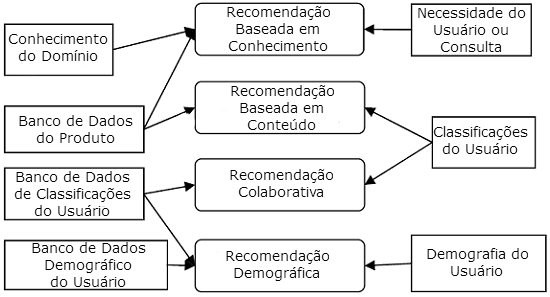
\includegraphics[scale=0.8]{imagens/recommendation_techniques_knowledg_sources.png}
	\caption{Técnicas de recomendação e suas fontes de conhecimento \citep{Burke:2007:HWR:1768197.1768211}.}
	\label{fig:tec_recomendacao_fontes_conhecimento}
\end{figure} 

	A seguir é discutido em detalhes alguns dos tipos de recomendação.
	
\subsection{Filtragem Colaborativa}

Na filtragem colaborativa o sistema recomenda ao usuário ativo itens que usuários com gostos similares gostaram no passado. A semelhança de gostos de dois usuários é calculada baseada na similaridade do histórico de classificações dos usuários. A filtragem colaborativa é considerada a técnica em sistemas de recomendação mais popular e mais largamente implementada \citep{ricci2011recommender}.

A ideia chave é que a classificação de um usuário \textit{u} para um novo item \textit{i} é provável de ser similar para a de outro usuário \textit{v}, se \textit{u} e \textit{v} tem classificado outros itens de maneira similar. De modo similar, é provável que \textit{u} classifique dois itens \textit{i} e \textit{j} de forma semelhante, se outros usuários tem feito classificações similares para estes dois itens \citep{ricci2011recommender}.

Em \cite{Burke:2002:HRS:586321.586352} e \cite{Burke:2007:HWR:1768197.1768211}, tem-se que os métodos de filtragem colaborativa podem ser divididos nas duas classes gerais baseados em \textit{vizinhança} e \textit{modelo}. Na filtragem colaborativa baseada em vizinhança as classificações usuário-item armazenadas no sistema são utilizadas diretamente para predizer classificações para novos itens. Isto pode ser feito de duas maneiras conhecidas como recomendação \textit{user-based} ou \textit{item-based} \citep{ricci2011recommender}.

Sistemas baseados em usuário, avaliam o interesse de um usuário \textit{u} por um item \textit{i} utilizando as classificações, para este item, de outros usuários, chamados \textit{vizinhos}, que tem padrões de classificação similar. Os vizinhos do usuário \textit{u} são tipicamente os usuários \textit{v} cujas classificações para os itens classificados por \textit{u} e \textit{v}, isto é I{$_{uv}$}, são mais correlacionados com aqueles de \textit{u}. A abordagem baseada no item, por outro lado, prediz a classificação de um usuário \textit{u} para um item \textit{i} baseado nas classificações de \textit{u} para itens similares a \textit{i}. Em tais abordagens, dois itens são similares se muitos usuários do sistema tem classificado estes itens de maneira similar \citep{ricci2011recommender}.

Diferente dos sistemas baseado em vizinhança, que usam as classificações armazenadas diretamente na predição, abordagens baseadas em modelo usam essas classificações para aprender um modelo preditivo. A ideia geral é modelar as interações usuário-item com fatores representando características latentes dos usuários e itens no sistema, como a classe de preferência do usuário e a classe de categoria dos itens. Este modelo é então treinado utilizando os dados disponíveis, e depois utilizado para predizer classificações de usuários para novos itens \citep{ricci2011recommender}.

\subsection{Filtragem Baseada em Conteúdo}

Sistemas de recomendação baseado em conteúdo tentam recomendar itens similares a aqueles que um usuário gostou no passado, ao passo que sistemas que utilizam o paradigma de recomendação colaborativa identificam usuários que possuem preferências similares a um usuário e recomenda itens que eles tem gostado \citep{lops2011ContentBased}.

\begin{figure}
	\centering
	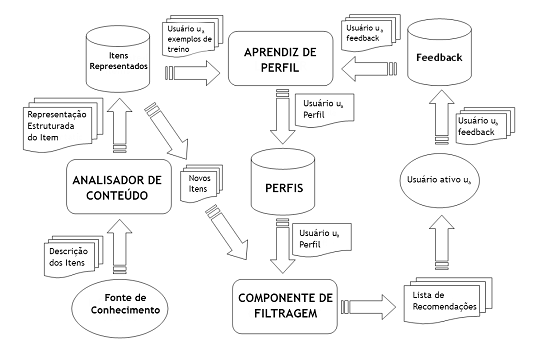
\includegraphics{imagens/content_based_architecture.png}
	\caption{Arquitetura de alto nível de um Sistema de Recomendação Baseado em Conteúdo \citep{lops2011ContentBased}.}
	\label{fig:content_based_architecture}
\end{figure} 

Sistemas implementando uma abordagem de recomendação baseada em conteúdo analisam um conjunto de documentos e/ou descrições de itens previamente classificados por um usuário, e constrói um modelo ou perfil de interesses do usuário baseado nas características dos objetos classificados por este usuário \citep{Mladenic:1999:TRI:630307.630472}. O perfil é uma representação estruturada dos interesses do usuário, adaptado para recomendar novos itens interessantes. O processo de recomendação consiste basicamente em combinar os atributos do perfil do usuário contra os atributos de um objeto de conteúdo. O resultado é um julgamento de relevância que representa os níveis de interesse do usuário naquele objeto. Se um perfil reflete com precisão as preferências do usuário, isso é uma grande vantagem para a eficácia no processo de acesso a informação. Por exemplo, poderia ser utilizado para filtrar os resultados de pesquisa para decidir se um usuário está interessado em uma específica página Web ou não e, em caso negativo, prevenir de ser exibida \citep{lops2011ContentBased}.

\subsection{Arquitetura de Sistemas de Recomendação Baseados em Conteúdo}

Segundo \cite{lops2011ContentBased}, em sistemas baseados em conteúdo é necessário utilizar técnicas apropriadas para representar os itens e produzir o perfil do usuário, e algumas estratégias para comparar o perfil do usuário com a representação do item. O processo de recomendação é realizado em três passos, cada qual é manipulado por um componente separado:

\begin{itemize}
	\item{\textbf{Analisador de Conteúdo}: Quando a informação não tem estrutura, como um texto, algum tipo de pré-processamento é preciso para extrair informação relevante e estruturada. A principal responsabilidade do componente é representar o conteúdo dos itens (por exemplo, documentos, páginas Web, notícias, descrição de produtos, etc.) vindos de fontes de informação de forma adequada para o próximo passo de processamento.}
	
	\item{\textbf{Aprendiz de Perfil}: Este módulo coleta dados representativos das preferências dos usuários e tenta generalizar estes dados, para construir o perfil do usuário. Normalmente, a estratégia de generalização é realizada através de técnicas de \textit{aprendizado de máquina}, que são capazes de inferir um modelo de interesses de usuário partindo de itens gostados ou não gostados no passado.}
	
	\item{\textbf{Componente de Filtragem}: Este módulo explora o perfil do usuário para sugerir itens relevantes através da combinação da representação do perfil do usuário contra os itens a serem recomendados. O resultado é um binário ou contínuo julgamento de relevância (computado utilizando alguma métrica de similaridade \citep{Herlocker:2004:ECF:963770.963772}), neste último caso resultando em uma lista ranqueada de itens potencialmente interessantes.}
\end{itemize}

A arquitetura de alto nível de um sistema de recomendação baseado em conteúdo está retratada na Figura \ref{fig:content_based_architecture}.


\subsection{Comparação das Técnicas de Recomendação}

Todas as técnicas de recomendação tem seus pontos fortes e fracos. \cite{Burke:2002:HRS:586321.586352} indicou alguns desses pontos, os quais são discutidos abaixo:

\begin{itemize}
	\item{\textbf{Usuário Novo}: Recomendações partem da comparação entre o usuário alvo e outros usuários baseado unicamente na acumulação de classificações, assim um usuário com poucas classificações é difícil de categorizar.}
	
	\item{\textbf{Item Novo}: Do mesmo modo, um item novo que não tem recebido muitas classificações também não pode ser facilmente recomendado: o problema do "item novo". É também conhecido como problema do "early rater", desde que a primeira pessoa a classificar um item recebe poucos benefícios por fazer isso. Isso torna necessário que sistemas de recomendação forneçam outros incentivos para encorajar usuários a fornecer classificações.}
\end{itemize}

Sistemas de recomendação colaborativos dependem das recomendações entre usuários e tem problemas quando o espaço de classificações é esparso, onde poucos usuários classificam os mesmos itens.

Estes três problemas sugerem que técnicas colaborativas puras são melhores para problemas onde a densidade de interesse do usuário é relativamente alta entre um pequeno e estático universo de itens. Se o conjunto de itens muda rapidamente, classificações antigas serão de pouco valor para novos usuários que não serão capazes de ter suas classificações comparadas com as dos usuários existentes. Se o conjunto de itens é grande e o interesse do usuário dissemina pouco, então a probabilidade de sobreposição com outros usuários será pequena \citep{Burke:2002:HRS:586321.586352}.

Sistemas de recomendação colaborativos funcionam melhor para um usuário que se encaixa em um nicho com muitos vizinhos de gosto semelhante. A técnica não funciona bem para o chamado "\textit{gray sheep}"~ \citep{claypool99}, que cai na fronteira entre panelinhas de usuários existentes. Isso também é um problema para sistemas demográficos que tentam categorizar usuários em características pessoais. Por outro lado, sistemas de recomendação demográficos não tem o problema do "usuário novo", porque eles não requerem um lista de classificações dos usuários. Ao invés, eles tem o problema de reunir as informações demográficas necessárias. \citep{Burke:2002:HRS:586321.586352}.

\section{Aplicações de Sistemas de Recomendação}

O primeiro sistema de recomendação foi um sistema experimental de filtragem de email, Tapestry \citep{goldberg1992tapestry}, desenvolvido por pesquisadores da Xerox Palo Alto Research Center \citep{Resnick:1997:RS:245108.245121}.

O objetivo do Tapestry era filtrar e arquivar os e-mails que chegavam todos os dias, de acordo com as opniões dadas pelas que efetuavam a leitura. Assim, este sistema utilizava uma abordagem colaborativa.

\subsection{TiVo}

Com o desenvolvimento das smart TVs, os usuários passaram a poder fazer classificações pela TV. TiVo\footnote{http://www.tivo.com} é um serviço de televisão muito utilizado nos Estados Unidos, que utiliza um sistema de recomendação para sugerir programas que sejam de interesse do usuário \citep{Ali:2004:TMS:1014052.1014097}. O TiVo permite que os usuários classifiquem os programas utilizando o controle remoto \ref{fig:tivo_recomendacao}.

O feedback implícito, por exemplo, se um filme está sendo gravado, é levado em consideração em adição da explícita classificação dos programas feita pelos usuários. Pedir ao usuários para responder perguntas é entediante e levanta questões de segurança, então o sistema tenta coletar as informações necessárias em background.

\begin{figure}
	\centering
	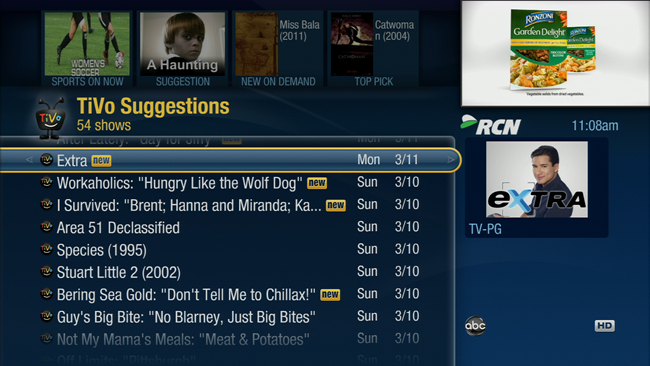
\includegraphics[scale=0.65]{imagens/TiVo_suggestion.png}
	\caption{Lista de Recomendação do Sistema de Recomendação do TiVo \citep{TiVoSuggestion}.}
	\label{fig:tivo_recomendacao}
\end{figure} 

O sistema do TiVo utiliza a Filtragem Colaborativa para fazer recomendações ao usuário com base nas preferências de usuários que tem gostos semelhantes. Também é utilizada a Filtragem Baseada em Conteúdo para fazer recomendações com base nas características (canal, título, gênero, atores) dos programas que o usuário já assistiu anteriormente.

\subsection{Biblioteca Digital}

Bibliotecas digitais são coleções de objetos digitais. Sistemas de Recomendação podem ser utilizados em uma aplicação de biblioteca digital para ajudar os usuários a localizarem e selecionarem informação e fontes de conhecimento \citep{Porcel:2010:DII:1663649.1663728}.

O CYCLADES\footnote{http://www.ercim.org/cyclades} \citep{rendaIPM05}, mostrado na Figura \ref{fig:cyclades}, é um ambiente colaborativo de arquivo virtual distribuído e aberto, que fornece diversos serviços para dar suporte a pesquisadores individuais como também a comunidade de pesquisadores, de uma maneira altamente personalizável. Os algoritmos de recomendação utilizam Filtragem Baseada em Conteúdo e Filtragem Colaborativa.


\begin{figure}
	\centering
	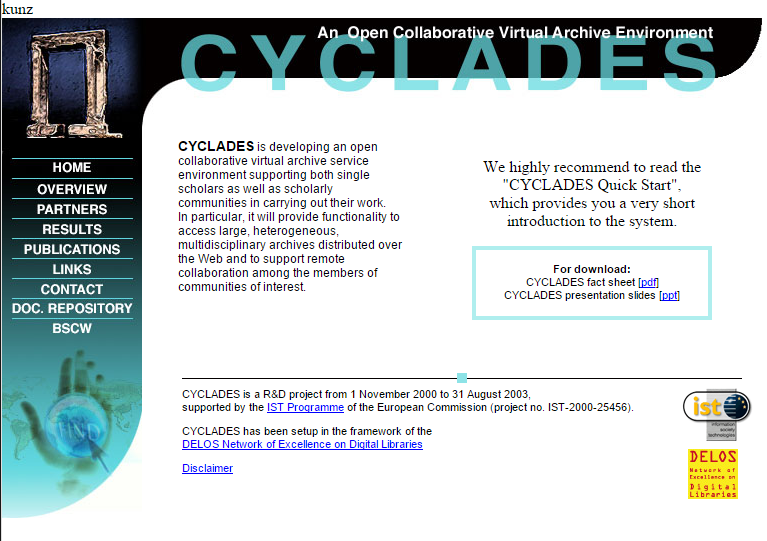
\includegraphics[scale=0.65]{imagens/cyclades.png}
	\caption{Página Web do CYCLADES. Figura elaborada pelo autor (2015).}
	\label{fig:cyclades}
\end{figure} 


\subsection{Amazon}

A Amazon\footnote{http://www.amazon.com} utiliza sistemas de recomendação para ajudar seus clientes a encontrar produtos para comprar \citep{Schafer:1999:RSE:336992.337035}.

\begin{figure}
	\centering
	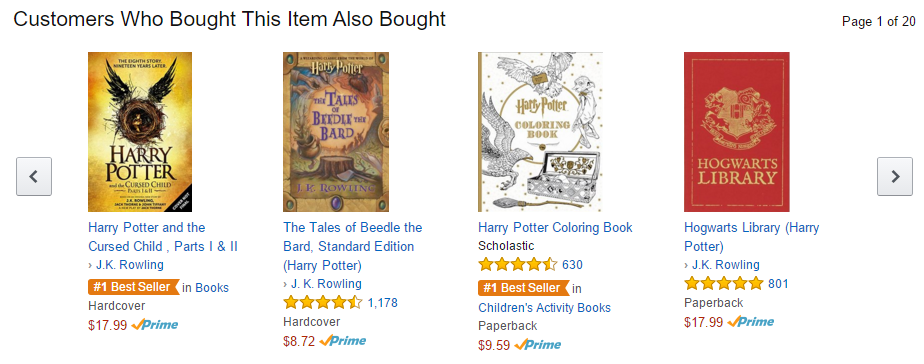
\includegraphics[scale=0.65]{imagens/amazon.png}
	\caption{Recomendação de Livros no site da Amazon. Figura elaborada pelo autor (2015).}
	\label{fig:amazon}
\end{figure} 

\textbf{Customers Who Bought This Item Also Bought}: a Amazon é estruturada com uma página de informação para cada livro, dando detalhes do texto e informação de compra. O recurso \textit{Clientes que compraram} é encontrado na página de cada livro do catálogo, e recomenda livros frequentemente comprados por clientes que compraram o livro selecionado. Na Figura \ref{fig:amazon} pode ser visto um exemplo em que são recomendados livros que foram comprados por clientes que também compraram um determinado livro.

\textbf{Amazon Delivers}: Clientes selecionam em uma lista de categorias/gênero, e periodicamente recebem e-mails com as últimas recomendações nas categorias escolhidas.

\textbf{Book Matcher}: Este recurso permite que clientes façam avaliação direta sobre livros que eles leram, onde dão notas em uma escala de 0 a 5. Depois de avaliar uma amostra de livros, os clientes podem solicitar recomendações de livros que podem gostar. Nesse ponto, uma meia dúzia de livros não-avaliados são apresentados os quais se relacionam com o gosto do usuário.

\textbf{Comentários dos Clientes}: Este recurso permite que clientes recebam recomendações de livros baseado nas opiniões de outros clientes. Está localizado na página de informação de cada livro, e é uma lista de 1-5 estrelas de avaliação com comentários fornecidos por outros clientes que leram o livro em questão.

\section{Sumário}

Neste capítulo, vimos uma visão geral sobre os Sistemas de Recomendação. Começamos mostrando um histórico sobre Sistemas de Recomendação. Em seguida discutimos alguns conceitos sobre os dados utilizados em um sistema. Então, foi apresentado uma lista de tarefas desempenhadas por sistemas de recomendação. Discutimos também as principais técnicas de recomendação. Por fim, foi mostrado algumas aplicações de sistemas de recomendação. No capítulo \ref{cap:userModel} discutiremos sobre o Modelo de Usuário. Será introduzido do que se trata, formas e requisitos de modelagem, e os principais algoritmos utilizados.